\documentclass[12pt]{article}
\usepackage[utf8]{inputenc}
\usepackage[T1]{fontenc}
\usepackage{amsmath}
\usepackage{graphicx}
\graphicspath{{.}}
\usepackage{listings}
\usepackage{hyperref}
\usepackage{color}
\usepackage{xcolor}
\usepackage{float}
\usepackage{tikz}
\usetikzlibrary{positioning}

% Code listing style
\lstset{
    language=C,
    basicstyle=\ttfamily\small,
    keywordstyle=\color{blue},
    stringstyle=\color{red},
    commentstyle=\color{green!60!black},
    numbers=left,
    numberstyle=\tiny,
    numbersep=5pt,
    frame=single,
    breaklines=true,
    breakatwhitespace=true,
}

\title{AxChain\\
\large CS 1412 - Final Project}
\author{Andres Antillon}
\date{December, 2024}

\begin{document}

\maketitle
\tableofcontents
\newpage

\section{Project Overview}
\subsection{Objectives}
This project aims to implement a minimalistic blockchain implementation in C. I'll avoid giving too much context as to how blockchains work, since that's not the main focus of the project. However, as this report explores many of the implementation details, it should be enough to understand the blockchain concepts being used.

The main objectives of this project were:
\begin{itemize}
    \item Implement core blockchain concepts including blocks, transactions, and mining
    \item Utilize secure cryptographic functions for transaction validation, verification, hashing and signing.
    \item Implement a deterministic address generation system
    \item Allow for chain persistence and reloading
\end{itemize}

\section{System Architecture}
\subsection{User Interface}
The system provides a terminal-based user interface with several key screens and components. It's the main way the user provides inputs and interacts with the system.

\subsubsection{Welcome Screen}
\begin{figure}[H]
\centering
\includegraphics[width=0.8\textwidth]{welcome_menu.png}
\caption{Initial welcome screen showing user initialization}
\end{figure}

The welcome screen (Figure 1) manages the initial user setup process. Users begin by entering a password for authentication. The system then generates a unique hexadecimal address (0x format) for the user's wallet. Upon successful initialization, the system displays the initial blockchain state, showing whether any existing chain data was loaded.

\subsubsection{Main Interface and Network Statistics}
\begin{figure}[H]
\centering
\includegraphics[width=0.8\textwidth]{main_menu.png}
\caption{Main interface showing network statistics and wallet information}
\end{figure}

The main interface (Figure 2) serves as the central dashboard for operations. 
Users can monitor network-wide statistics including the total number of transactions, 
active account count, and total AX token supply. The interface displays the user's 
wallet information, showing their unique address and current AX token balance. 
A navigation menu with intuitive icons provides access to core functions like 
sending tokens, mining, and viewing the chain.

\subsubsection{Transaction Interface}
\begin{figure}[H]
\centering
\includegraphics[width=0.8\textwidth]{transaction_menu.png}
\caption{Transaction interface showing validation and error handling}
\end{figure}

The transaction interface (Figure 3) handles all token transfer operations. It implements comprehensive validation to ensure transaction integrity. All recipient addresses must follow the 0x format specification. The system validates token amounts against the sender's available balance. Real-time debugging information and clear error messages guide users through the transaction process, helping them correct any input errors immediately.

\subsubsection{Mining Interface}
\begin{figure}[H]
\centering
\includegraphics[width=0.6\textwidth]{mining_menu}
\caption{Mining interface showing proof-of-work process}
\end{figure}

The mining interface (Figure 4) provides real-time feedback during the block mining process. Users can monitor the current mining difficulty, represented by the required number of leading zeros in the hash. The interface displays a live counter of hash attempts and notifies users when a block is successfully mined. Upon success, it shows the final block hash and confirms the mining reward amount.

\subsubsection{Chain History}
\begin{figure}[H]
\centering
\includegraphics[width=0.6\textwidth]{history_menu}
\caption{Transaction history view showing blockchain state}
\end{figure}

The chain history view (Figure 5) offers a comprehensive overview of all blockchain activity. Users can view the complete transaction history, with each entry containing detailed timestamp information. The view displays transaction hashes and their links to previous transactions, enabling verification of the chain's integrity. A transaction counter helps users track the total number of operations in the blockchain.

\subsubsection{Chain Persistence}
The blockchain state is maintained through a binary data file (axchain.dat) that serves as persistent storage. This file:
\begin{itemize}
\item Stores the complete transaction history in a binary format
\item Is automatically loaded when the application starts
\item Updates in real-time as new transactions are mined
\item Enables multiple instances to share the same chain state
\item Maintains data integrity through hash-linked transactions
\end{itemize}

The data file allows the blockchain to persist between sessions and enables decentralized operation, where multiple users can interact with the same chain through the shared file system.

\subsection{Function Structure}
\begin{figure}[h]
\centering
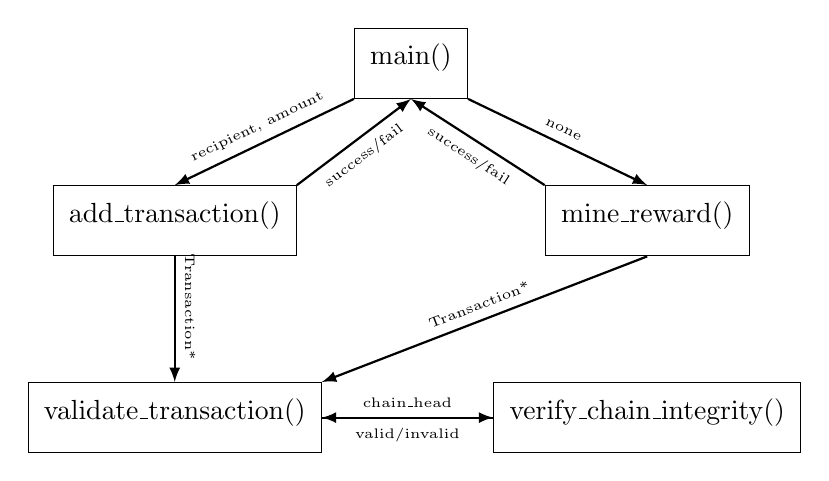
\begin{tikzpicture}[
    module/.style={
        draw,
        rectangle,
        minimum height=8mm,
        text depth=1.5ex,
        inner sep=2mm,
        align=center
    },
    flow/.style={
        ->,
        >=latex,
        thick
    },
    label/.style={
        font=\tiny,
        sloped,
        anchor=center
    }
]
    % Main program layer
    \node[module] (main) at (0,4) {main()};
    
    % Core operations layer (moved down more)
    \node[module] (add) at (-3,2) {add\_transaction()};
    \node[module] (mine) at (3,2) {mine\_reward()};
    
    % Validation layer (moved down more)
    \node[module] (validate) at (-3,-0.5) {validate\_transaction()};
    \node[module] (verify) at (3,-0.5) {verify\_chain\_integrity()};
    
    % Draw connections from main with more space
    \draw[flow] (main.south west) -- node[label, above] {recipient, amount} (add.north);
    \draw[flow] (main.south east) -- node[label, above] {none} (mine.north);
    
    % Core operation flows with adjusted spacing
    \draw[flow] (add.south) -- node[label, above, pos=0.4] {Transaction*} (validate.north);
    \draw[flow] (mine.south) -- node[label, above] {Transaction*} (validate.north east);
    
    % Validation flows
    \draw[flow] (validate) -- node[label, above] {chain\_head} (verify);
    \draw[flow] (verify) -- node[label, below] {valid/invalid} (validate);

    % Return flows with more space
    \draw[flow] (add.north east) -- node[label, below] {success/fail} (main.south);
    \draw[flow] (mine.north west) -- node[label, below] {success/fail} (main.south);

\end{tikzpicture}
\caption{Function call hierarchy and data flow in the blockchain implementation}
\end{figure}

This function call hierarchy and data flow diagram (Figure 6) paints a very broad overview of the system. It shows the main functions that the UI calls, however, it fails to describe the underlying function calls that each makes in order to perform their function. Yet, I believe this is enough to describe how the system interfaces with other functions since most underlying functions do not have any dependencies.

\newpage
\section{Implementation Details}

\subsection{Core Components}
The implementation consists of a linked list of transactions, where each transaction contains:

\begin{lstlisting}[language=C]
typedef struct Transaction {
    char sender[65];      // Sender's address
    char recipient[65];   // Recipient's address  
    double amount;        // Transfer amount
    double fee;          // Transaction fee
    time_t timestamp;    // Creation time
    char prev_hash[65];  // Previous transaction's hash
    char data_hash[65];  // Hash of transaction data
    char signature[129]; // Transaction signature
    struct Transaction* next;  // Next in chain
} Transaction;
\end{lstlisting}

\subsection{Function Documentation}

\subsubsection{Core Transaction Operations}
% Core transaction handling
\textbf{add\_transaction}

Description: Creates and adds a new transaction to the chain. Validates the recipient address, checks sender's balance, performs proof-of-work, and adds the transaction to the chain if valid.

Parameters:
\begin{itemize}
\item recipient: Target address in 0x... format
\item amount: Amount to transfer (must be > 0)
\end{itemize}

Returns: 1 on success, 0 on failure

\vspace{1em}
\hrule
\vspace{1em}

\textbf{validate\_transaction}

Description: Performs comprehensive transaction validation including address format, balance checks, signature verification, and mining reward validation.

Parameters:
\begin{itemize}
\item Transaction* tx: Pointer to transaction to validate
\end{itemize}

Returns: 1 if valid, 0 if invalid

\vspace{1em}
\hrule
\vspace{1em}

\textbf{verify\_chain\_integrity}

Description: Validates the entire blockchain by traversing the linked list for:
\begin{itemize}
\item Valid transaction formats
\item Correct mining rewards
\item Valid address formats
\item Proper chain linking between nodes
\end{itemize}

Parameters: None

Returns: 1 if chain is valid, 0 if corrupted

\vspace{1em}
\hrule
\vspace{1em}

\textbf{is\_double\_spend}

Description: Checks if a transaction is a double spend by verifying the transaction's hash against the chain's history.

Parameters:
\begin{itemize}
\item Transaction* tx: Pointer to transaction to check
\end{itemize}

Returns: 1 if double spend, 0 if not

\vspace{1em}
\hrule
\vspace{1em}

\textbf{validate\_address}

Description: Checks if an address format is valid.

Parameters:
\begin{itemize}
\item const char* address: Address to validate
\end{itemize}

Returns: 1 if valid, 0 if invalid

\vspace{1em}
\hrule
\vspace{1em}

\textbf{get\_mining\_reward\_count}

Description: Counts total number of mining rewards issued in the chain by traversing the linked list of transactions.

Parameters: None

Returns: \texttt{size\_t} - Number of mining rewards

\vspace{1em}
\hrule
\vspace{1em}

\textbf{get\_total\_fees\_burned}

Description: Calculates total transaction fees that have been burned by traversing the linked list of transactions.

Parameters: None

Returns: double - Total amount of fees burned

\vspace{1em}
\hrule
\vspace{1em}

\subsubsection{Mining Operations}
\textbf{mine\_reward}

Description: Mines a new reward transaction:
\begin{itemize}
\item Creates transaction with BLOCKCHAIN\_REWARD sender
\item Sets reward amount to MINING\_REWARD
\item Performs proof-of-work
\item Adds to chain if successful
\end{itemize}

Parameters: None

Returns: void

\vspace{1em}
\hrule
\vspace{1em}

\subsubsection{Account Management}
\textbf{initialize\_user}

Description: Creates or loads user's cryptographic identity:
\begin{itemize}
\item Generates RSA key pair from password
\item Derives user's address from public key
\item Stores keys for transaction signing
\end{itemize}

Parameters:
\begin{itemize}
\item const char* password: User's password for key generation
\end{itemize}

Returns: void

\vspace{1em}
\hrule
\vspace{1em}

\textbf{get\_current\_user\_address}

Description: Returns the current user's blockchain address.

Parameters: None

Returns: const char* - String containing user's address (0x... format)

\vspace{1em}
\hrule
\vspace{1em}

\textbf{get\_account\_balance}

Description: Calculates account balance by traversing the linked list of transactions and summing all transactions involving the address.

Parameters:
\begin{itemize}
\item const char* address: Account address to check
\end{itemize}

Returns: double - Current balance in AX

\vspace{1em}
\hrule
\vspace{1em}

\subsubsection{Chain State Functions}
\textbf{get\_chain\_head}

Description: Returns the head pointer of the blockchain linked list.

Parameters: None

Returns: Transaction* - Pointer to the head of the blockchain

\vspace{1em}
\hrule
\vspace{1em}

\textbf{get\_transaction\_count}

Description: Returns total number of transactions in the chain.

Parameters: None

Returns: \texttt{size\_t} - Number of transactions

\vspace{1em}
\hrule
\vspace{1em}

\textbf{get\_active\_accounts}

Description: Counts unique addresses that have participated in transactions by traversing the linked list of transactions.

Parameters: None

Returns: \texttt{size\_t} - Number of active accounts

\vspace{1em}
\hrule
\vspace{1em}

\textbf{get\_total\_supply}

Description: Calculates total currency in circulation by summing all mining rewards by traversing the linked list of transactions.

Parameters: None

Returns: double - Total supply of AX tokens

\vspace{1em}
\hrule
\vspace{1em}

\textbf{get\_chain\_modified\_time}

Description: Gets the last modification time of the chain file.

Parameters: None

Returns: \texttt{time\_t} - Last modification timestamp, or 0 if file doesn't exist

\vspace{1em}
\hrule
\vspace{1em}

\textbf{cleanup\_chain}

Description: Frees all memory associated with the blockchain by traversing the linked list of transactions:
\begin{itemize}
\item Iterates through all transactions in the chain
\item Frees each transaction node
\item Resets chain head pointer
\end{itemize}

Parameters: None

Returns: void

\vspace{1em}
\hrule
\vspace{1em}

\textbf{has\_chain\_changed}

Description: Monitors blockchain file for updates from other instances:
\begin{itemize}
\item Checks modification time
\item Throttles checks to once per second
\item Handles file existence
\end{itemize}

Parameters: None

Returns: 1 if chain needs reload, 0 if chain is current

\subsubsection{Cryptographic Operations}
\textbf{generate\_hash}

Description: Creates SHA256 hash of input data:
\begin{itemize}
\item Used for mining proof-of-work
\item Transaction data hashing
\item Chain linking
\end{itemize}

Parameters:
\begin{itemize}
\item const void* data: Data to hash
\item size\_t len: Length of data
\item char* output: Buffer for hex string output
\end{itemize}

Returns: void

\vspace{1em}
\hrule
\vspace{1em}

\textbf{sign\_transaction}

Description: Signs a transaction using the sender's private key:
\begin{itemize}
\item Creates transaction data hash
\item Signs hash with RSA private key
\item Stores hex signature in transaction
\end{itemize}

Parameters:
\begin{itemize}
\item Transaction* tx: Transaction to sign
\end{itemize}

Returns: void

\vspace{1em}
\hrule
\vspace{1em}

\textbf{verify\_transaction}

Description: Verifies transaction signature by:
\begin{itemize}
\item Reconstructing transaction data hash
\item Verifying RSA signature
\item Validating against sender's public key
\end{itemize}

Parameters:
\begin{itemize}
\item Transaction* tx: Transaction to verify
\end{itemize}

Returns: 1 if signature valid, 0 if verification fails

\subsubsection{Persistence Operations}
\textbf{save\_chain}

Description: Handles blockchain persistence with:
\begin{itemize}
\item Version checking
\item Checksum validation
\item Atomic file updates
\item Chain integrity verification
\end{itemize}

Parameters: None

Returns: 1 on success, 0 on any error

\vspace{1em}
\hrule
\vspace{1em}

\textbf{load\_chain}

Description: Loads and validates the blockchain from disk

Parameters: None

Returns: 1 on success, 0 on any error

\vspace{1em}
\hrule
\vspace{1em}

\newpage
\section{Testing}

\subsection{Test Plan}
The testing strategy focused on three key areas, implemented in \texttt{tests.c}:

\subsubsection{Unit Tests}
\begin{itemize}
\item \textbf{Mining Operations}
    \begin{itemize}
    \item Reward transaction creation
    \item Balance crediting accuracy
    \item Transaction structure validation
    \item Mining difficulty verification
    \end{itemize}
\item \textbf{Transaction Validation}
    \begin{itemize}
    \item Balance sufficiency checks
    \item Address format validation
    \item Amount validation
    \item Fee calculation accuracy
    \end{itemize}
\item \textbf{Chain Integrity}
    \begin{itemize}
    \item Empty chain validation
    \item Post-mining chain state
    \item Post-transaction verification
    \item Hash linking verification
    \end{itemize}
\end{itemize}

\subsection{Test Results}
Test execution produced the following results:

\subsubsection{Mining Tests}
\begin{itemize}
\item Successfully verified mining reward of \texttt{MINING\_REWARD} AX
\item Confirmed correct transaction structure:
    \begin{itemize}
    \item Sender set to "BLOCKCHAIN\_REWARD"
    \item Recipient matches miner's address
    \item Amount matches defined reward
    \item Valid proof-of-work hash
    \end{itemize}
\item Validated balance updates after mining
\end{itemize}

\subsubsection{Transaction Tests}
\begin{itemize}
\item Successfully validated legitimate transactions
\item Properly rejected invalid scenarios:
    \begin{itemize}
    \item Insufficient balance attempts
    \item Malformed addresses
    \item Zero-amount transfers
    \end{itemize}
\item Verified balance deductions including fees
\item Confirmed transaction signature verification
\end{itemize}

\subsubsection{Chain Integrity Tests}
\begin{itemize}
\item Validated empty chain state
\item Verified chain integrity after mining operations
\item Confirmed integrity after transaction additions
\item Tested hash linking between transactions
\end{itemize}

\begin{figure}[H]
    \centering
    \includegraphics[width=0.8\textwidth]{test_results.png}
    \caption{Test execution output showing all test cases passing}
\end{figure}

\subsection{Test Framework}
The testing framework implements several assertion functions:
\begin{itemize}
\item \texttt{assert\_true}: Basic boolean condition testing
\item \texttt{assert\_equal\_double}: Floating-point comparison with epsilon
\item \texttt{assert\_equal\_str}: String equality verification
\end{itemize}

Test results are tracked using a \texttt{TestResults} structure that maintains:
\begin{itemize}
\item Total tests run
\item Number of passed tests
\item Number of failed tests
\end{itemize}

The framework provides clear visual feedback using:
\begin{itemize}
\item check for passed tests
\item cross for failed tests
\item Detailed error messages for failures
\end{itemize}

\section{Analysis and Observations}

\subsection{Successful Aspects}
I was able to succesfully implement a blockchain implementation that, while not fully complete, achieves all of the objectives of the project. The use of external libraries, such as OpenSSL, made it easier to implement the crucial cryptographic operations. While I can not take full credit for their implementation, I was able to implement the exact functions I required. It was particularly satisfying to see how I was able to adapt the concepts of blockchains to fit something much more manageable, such as the focus on individual transactions rather than full blocks and the account management system using passwords. This allowed me to implement a system that still performs as a blockchain would usually perform but in a much more approachable and easy to understand way.

\subsection{Implementation Challenges}
The original scope of this project went beyond even a simple blockchain implementation. However, even after having made great progress, I eventually ran into issues which made it virtually impossible to continue with that version. Thankfully, that process was incredibly informative and educational. It allowed me to learn about all the technical considerations that go into implementing a blockchain, particularly using the C programming language. This made it much easier when I eventually had to switch to a more manageable version. I was able to begin from scratch with a much clearer understanding of what was needed, but more importantly, what was not needed.

\subsection{Future Improvements}
There are a number of improvements I wish to make. Even more so, considering that I had to narrow the scope of the project quite a bit from what I originally had in mind. I would like to implement:
\begin{itemize}
\item A networking layer to allow multiple clients, from different machines, to interact with the blockchain.
\item The ability to send messages over transactions, such as a message from one user to another.
\item A more comprehensive mining system to allow for a more interesting behaviour with the tokens.
\end{itemize}

\end{document} 